\documentclass{article}

% if you need to pass options to natbib, use, e.g.:
%     \PassOptionsToPackage{numbers, compress}{natbib}
% before loading neurips_2020

% ready for submission
% \usepackage{neurips_2020}

% to compile a preprint version, e.g., for submission to arXiv, add add the
% [preprint] option:
%     \usepackage[preprint]{neurips_2020}

% to compile a camera-ready version, add the [final] option, e.g.:
%     \usepackage[final]{neurips_2020}

% to avoid loading the natbib package, add option nonatbib:
     \usepackage[final, nonatbib]{neurips_2020}

\usepackage[utf8]{inputenc} % allow utf-8 input
\usepackage[T1]{fontenc}    % use 8-bit T1 fonts
\usepackage{hyperref}       % hyperlinks
\usepackage{url}            % simple URL typesetting
\usepackage{booktabs}       % professional-quality tables
\usepackage{amsfonts}       % blackboard math symbols
\usepackage{nicefrac}       % compact symbols for 1/2, etc.
\usepackage{microtype}      % microtypography
\usepackage{multirow}
\usepackage{makecell}
\usepackage{csquotes}
\usepackage{graphicx}

\title{Security and Privacy of Machine Learning - Homework 2}

\author{
  Wu-Jun Pei\\
  National Taiwan University\\
  \texttt{b06902029@ntu.edu.tw} \\
}

\begin{document}

\maketitle

\begin{abstract}
Despite the mightiness of deep nerual networks, several studies have shown that they are vulnerable
to adversarial examples. In this homework, we tried to build a black-box defense on CIFAR-10.
Finally, my adversarially trained ensemble model with a vanilla JPEG compression as a preprocessing
could defend well against strong attacks.
\footnote{Due to page limit, I will skip contents that can be found in the homework specs.}
\end{abstract}

\section{Introduction}

As suggested in class \cite{spml0925}, we should state the considered threat model
precisely. The threat model I consider is listed as below:

\begin{itemize}
  \item The adversary has limited knowledge of the model, he only knows the model architecture, but
  is totally ignorant of the training process and the model weights.
  \item The adversary can perturb each pixel up to 8 (in 0-255 scale).
\end{itemize}

\section{Methods}
\subsection{Adversarial Training}
\subsubsection{Modified Adversarial Training}
Adversarial training \cite{madry2019deep} may take a long time, and it's mostly from
\textit{generating adversarial examples}. In this homework, to reduce computational cost and fasten
the adversarial training, I modified a step the adversarial training. During adversarial training,
for an input $x$, we used to generate adversarial examples $x'$ in that optimization step and train
the model with $x'$. However, it would be wasting if the model hadn't learned from the adversarial
examples. Thus, I store $x'$ and reuse them for several epochs.

\subsubsection{Adversarial Training on Ensemble Models}
\label{section:adv-training-on-ensemble-models}
In addition to the natural property of adversarial attack, adversarial attacks on a ensemble model
would take even more time since each model has to forward the input once. To overcome the
computational cost, I redesign the adversarial training process. Whenever the adversarial examples
need to be regenerated, instead of attacking directly on the ensemble model, we attack on a submodel
in the ensemble model that is chosen at random. Although not tested thoroughly, the mechanism should
work because of the transferbility of adversarial attacks between models.

\subsection{Preprocessing-based Defenses}
In my previous homework, I've already shown that some preprocessing-based defenses, such as vanilla
JPEG Compression, are effective enough to eliminate the influence of adversarial perturbations. In
this homework, I'm going to explore defenses that are more effective.

\subsubsection{Baseline}
Inspired by the preprocessing method TA used in the evaluation of previous homework, I setup the
baseline method as: \textbf{ColorJitter} (brightness = 0.4, contrast = 0.4, saturation = 0.4, hue =
0.25) $\to$ \textbf{CenterCrop} (size = 24) $\to$ \textbf{Pad} (size = 4)

\subsubsection{Vanilla JPEG Compression}
We apply JPEG Compression on the entire image before feeding it to our model in order to reduce the
adversarial noise.

\subsubsection{SHIELD}
Similar to \textit{Vanilla JPEG Compression}, we divide the image into several equal sized
subimages. For each subimage, we apply different JPEG quality at random on it. And finally, we
concatenate the compressed subimages back.

\subsection{Evalution}
\label{section:evaluation}
To evaluate my work fairly, I unify the method to evaluate each model. Specifically, we create
several adversarial datasets for evaluation in the following settings:
\begin{itemize}
  \item The proxy models are \texttt{nin}, \texttt{resnet20}, \texttt{sepreresnet56},
  \texttt{densenet40-k12-bc}, and \texttt{diaresnet110}.
  \item PGD attack, constrained to $l_2$ norm $\epsilon = 8 / 256$
  \item The number of iterations could be 8, 16, 32, 64 and 128.
\end{itemize}

\section{Experiments and Findings}

\subsection{Adversarial Training Epochs}
\paragraph{Experiment Settings} In this experiment, we want to examine if increasing adversarial
training epochs improves the general adversarial accuracy. The model we used is \texttt{resnet20}
since it's more lightweight. We regenerate new adversarial examples every epoch, and each
adversarial example is generated with 8 iterations of PGD attack. We evaluate the model with
adversarial sets with different attack strengthes.

\paragraph{Findings} The experiment results are shown in figure \ref{img:exp-training-epochs}. We
can see that the model improves a lot in the first two epochs, and have no significant improvement
on evaluation set afterwards. Also, we can see that training on adversarial examples generated with
8 iterations have a fair performance on all other evaluation sets generated with larger iterations.
These findings suggest us that we can adversarially train our model with weaker adversarial set and
with less training epochs, saving computational costs. Although it seems robust to the evaluation
adversarial set, it's still vulnerable if the attacker knows the model weights. The accuracy on
newly generated adversarial examples are about 15\% on the last epoch.

\begin{figure}[ht]
  \begin{center}
  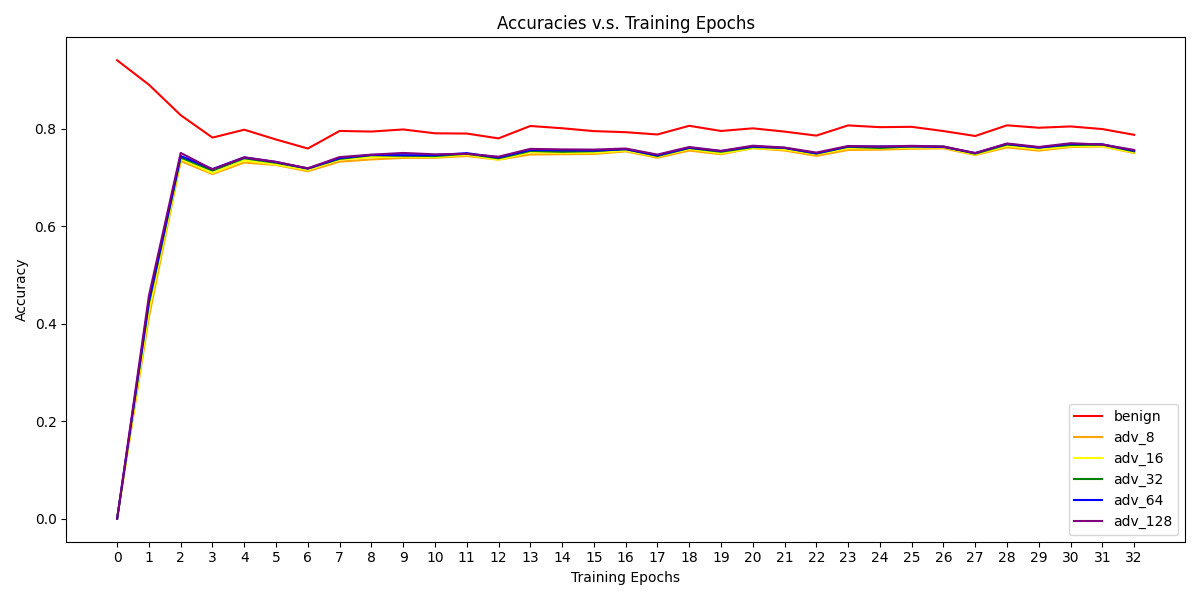
\includegraphics[width=0.8\linewidth]{imgs/exp-training-epochs.png}
  \end{center}
  \caption{\texttt{resnet20}'s accuracies on different training epoch, evaluated on adversarial sets
  generated with different number of iterations}
  \label{img:exp-training-epochs}
\end{figure}

\subsection{Preprocessing-based Defenses}
\paragraph{Experiment Settings} To test the effectivness of those defenses, I used two pretrained
\texttt{pytorchcv} models (without adversarial training), \texttt{resnet20} and \texttt{resnet1001}.
The adversarial examples are generated as described in section \ref{section:evaluation}
with 16 iterations of PGD.

\paragraph{Findings} The experiment results are shown in table
\ref{experiment:pgd-iterations}. We can see similar performance on the two models. The
baseline method has little effect on adversarial examples, while both vanilla JPEG compression and
SHIELD are more effective. To take a closer glimpse, we can see that vanilla JPEG compression method
has better on both benign set and adversarial set. I guess that it may result from that the image
size in CIFAR-10 is already small (32x32), and the smaller splitted images will not benefit from the
JPEG compression.

\begin{table}[ht]
  \label{experiment:pgd-iterations}
  \centering
  \caption{Evaluation of different preprocessing based defense. The plus sign (+) indicates the
    benign set while the minus sign (-) indicates the adversarial set.}
  \begin{tabular}{ccccccccc}
    \toprule
    & \multicolumn{4}{c}{resnet20} & \multicolumn{4}{c}{resnet1001} \\
    \cmidrule(r){2-5} \cmidrule(r){6-9}
    Defense Method            & Train + & Train - & Val. +  & Val. -  & Train + & Train - & Val. +  & Val. -  \\
    \midrule
    None                      & 0.9865  & 0.0000  & 0.9403  & 0.0001  & 1.0000  & 0.3962  & 0.9672  & 0.3420  \\
    Baseline                  & 0.8622  & 0.1957  & 0.8181  & 0.1950  & 0.9403  & 0.4847  & 0.8792  & 0.4462  \\
    JPEG (quality = 60)       & 0.8211  & 0.6389  & 0.7924  & 0.6162  & 0.9257  & 0.8239  & 0.8671  & 0.7563  \\
    SHIELD (block size = 4)   & 0.7917  & 0.5902  & 0.7634  & 0.5688  & 0.8939  & 0.7719  & 0.8322  & 0.7068  \\
    \bottomrule
  \end{tabular}
\end{table}


\section{Final Model}
\paragraph{Model Architecture} Ensemble (by averaging the output) model of \texttt{nin},
\texttt{resnet20}, \texttt{sepreresnet56}, \texttt{densenet40-k12-bc} and \texttt{diaresnet110}.
The model architectures and initial weights are credited to \texttt{pytorchcv}\cite{imgcls}. The most important
reason I adopt an ensemble model is that it's believed ensemble model could resolve the problem
when only one model misfunctions. It's quite useful when we consider the robustness of a model.
\paragraph{Adversarial Training} Adversarial training on ensemble models as described in
section \ref{section:adv-training-on-ensemble-models}. The model is trained with 256 epochs, and
adversarial examples are regenerated every 4 epochs, using PGD attacks with 16 iterations. The
entire training process takes about 32 hours on a single RTX 2070 Super.
\paragraph{Preprocessing-based Defense} Among many effective methods, I applied
\textbf{Vanilla JPEG Compression} with quality = 60 since it's effective without harming the
benign accuracy too much.

\subsection{Analysis and Findings}

\paragraph{Training Log} The training log is shown on figure \ref{img:final-training-log}. The
sudden drops on adversarial accuracies are due to that new adversarial examples were effective and
made the ensemble output the wrong answer. Also, we can observe that attacking on a single
\texttt{sepreresnet56} was significantly more successful than others. It's possibly because that
it's so similar to the ensemble model. I also tested the performance on different adversarial
dataset.

\begin{figure}[ht]
  \centering
  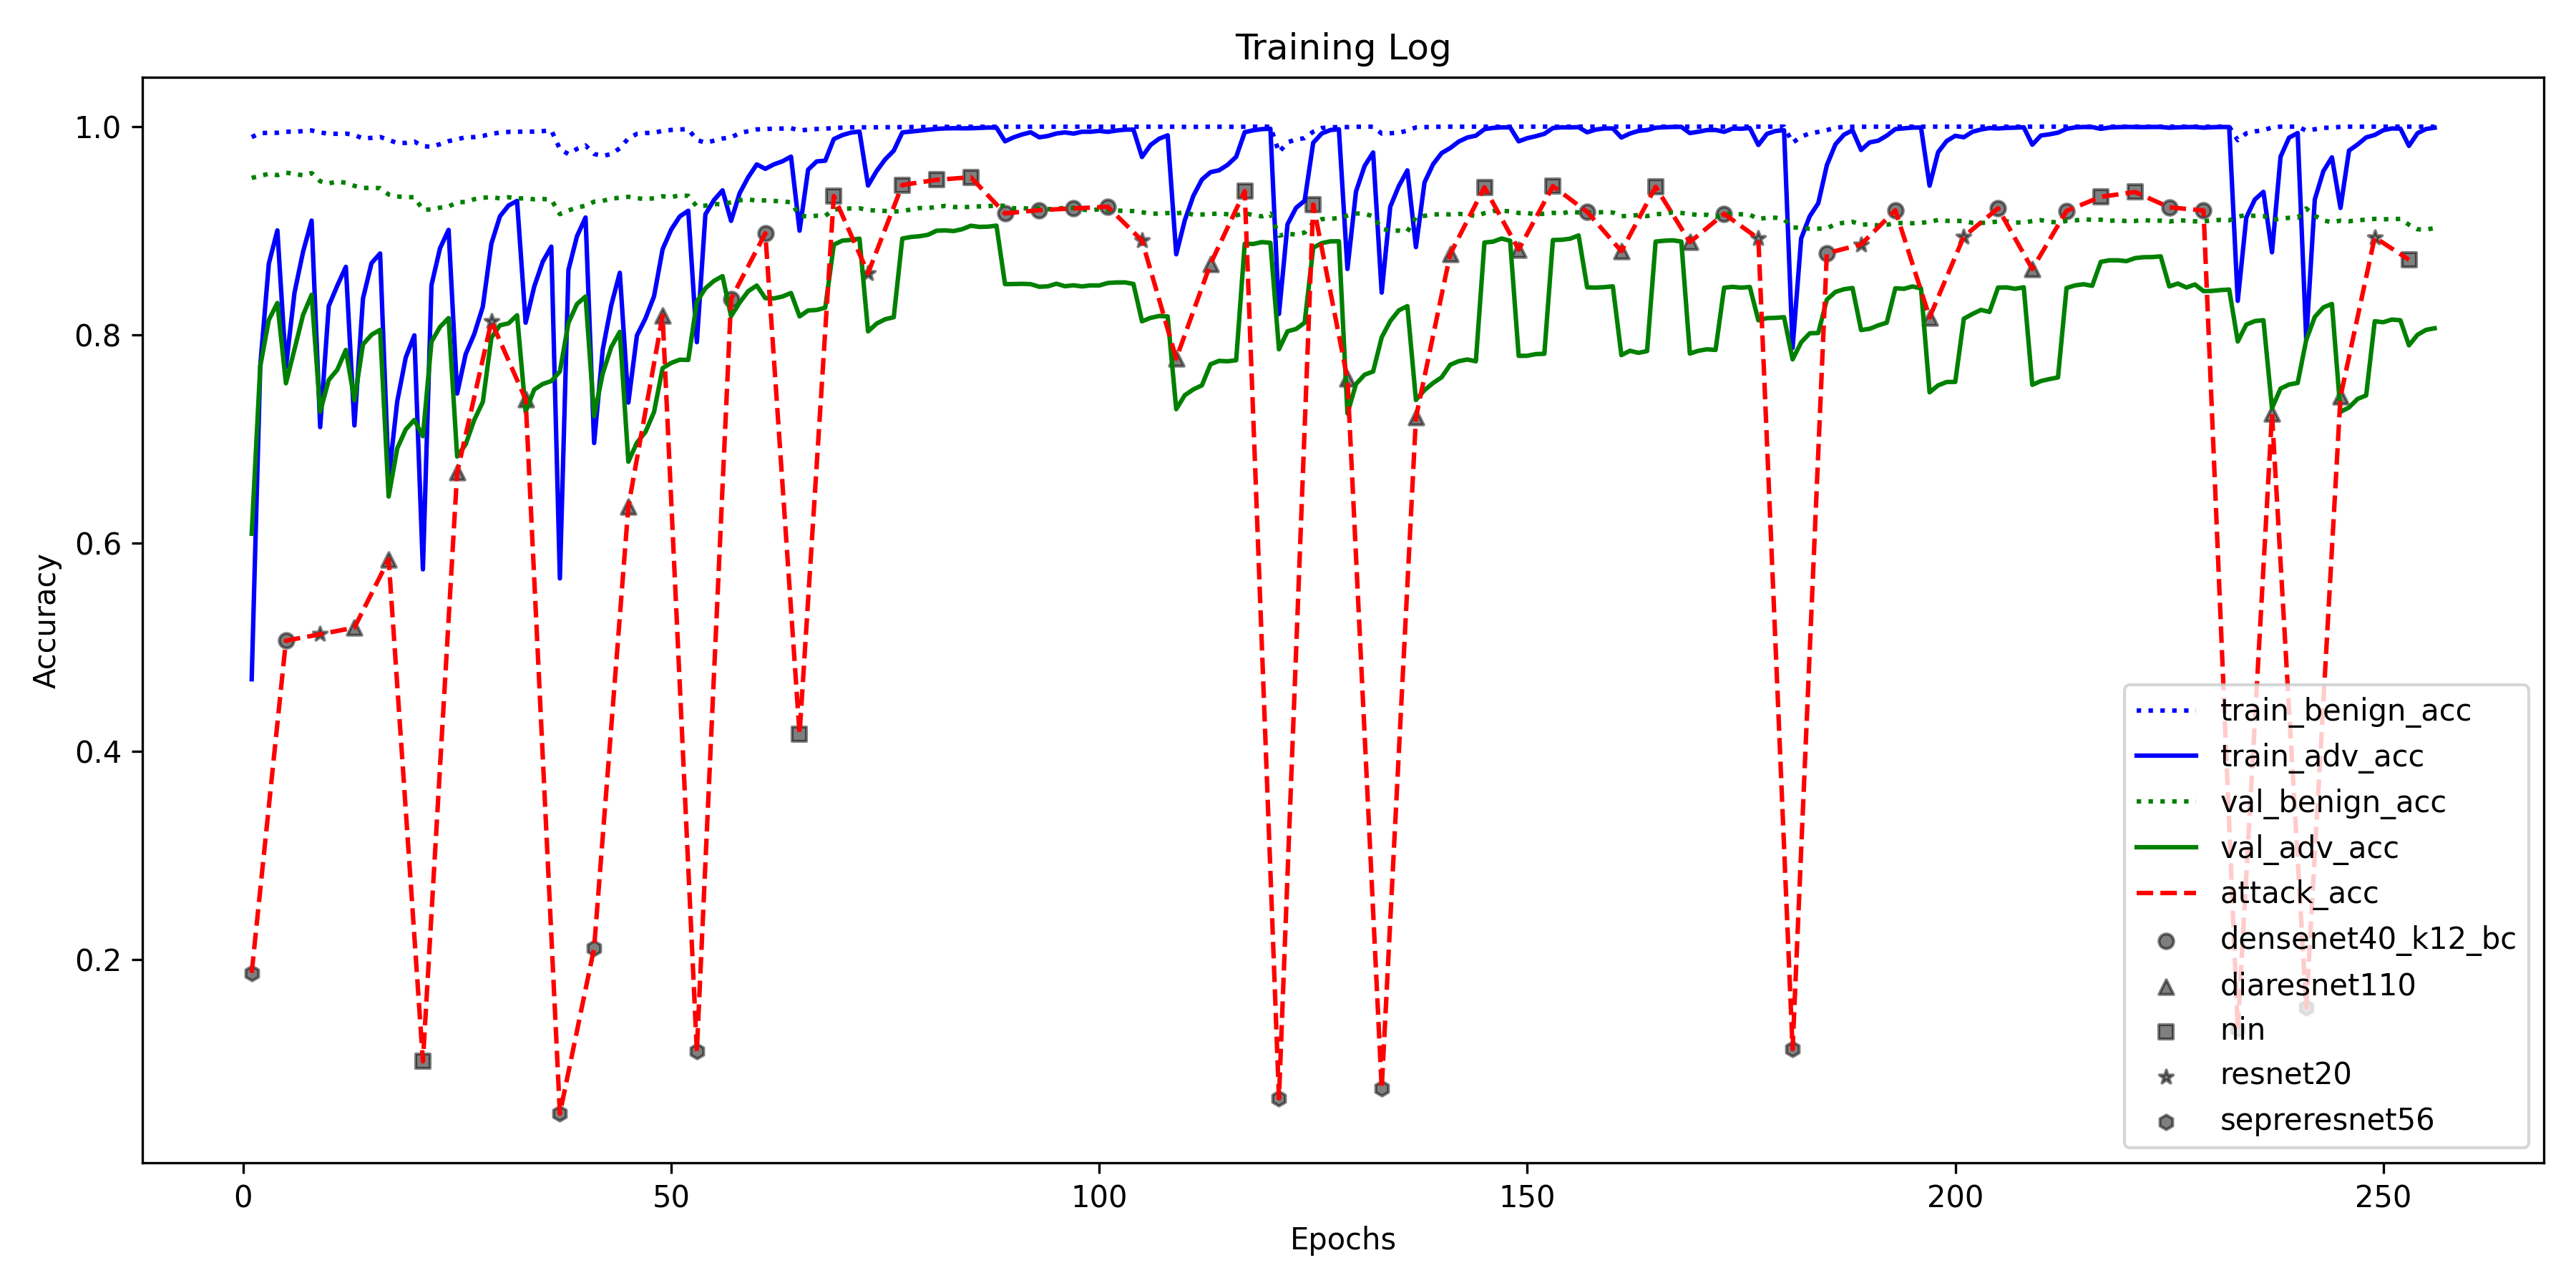
\includegraphics[width=0.8\linewidth]{imgs/final-training-log.png}
  \caption{Training log of my ensemble model}
  \label{img:final-training-log}
\end{figure}

\begin{figure}[ht]
  \centering
  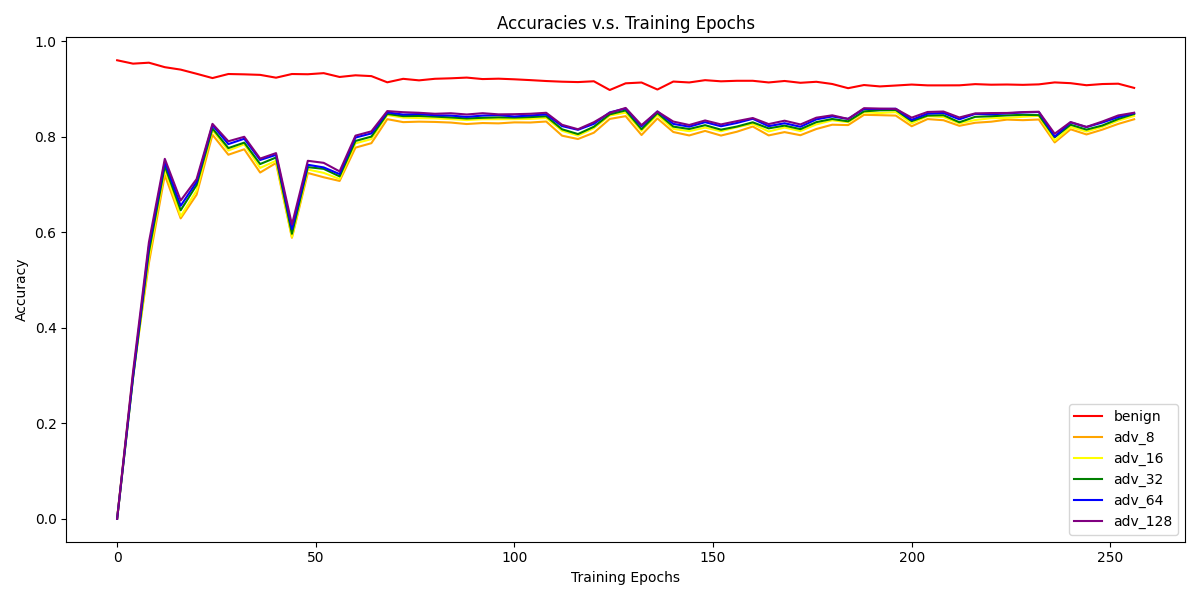
\includegraphics[width=0.8\linewidth]{imgs/final-evaluation.png}
  \caption{Evaluation on different epochs of my ensemble model}
  \label{img:final-evalution}
\end{figure}


\paragraph{Evaluation} The evaluation results are shown on table \ref{table:eval-ensemble-model}. We
can easily see that our model performs well on both benign dataset and adversarial datasets with
accuracies greater than 80\%. Also, it's worth noting that the ensemble proxy model we attacked on
is the same as the ensemble model we utilize here. This implies that even the adversary has access
to our model, they cannot attack our model effectively. As for the defense, we cans see that
applying it does not help the either benign accuracy nor adversarial accuracy; however, I'll
consider it as a part of my model as a safety guard.

\begin{table}[ht]
  \label{table:eval-ensemble-model}
  \centering
  \caption{Evaluation of our ensemble model.}
  \begin{tabular}{ccccccc}
    \toprule
    Defense                   & Benign  & Adv-8   & Adv-16  & Adv-32  & Adv-64  & Adv-128 \\
    \midrule
    None                      & 0.9026  & 0.8369  & 0.8437  & 0.8479  & 0.8498  & 0.8506  \\
    Vanilla JPEG Compression  & 0.8688  & 0.8303  & 0.8363  & 0.8398  & 0.8399  & 0.8431  \\
    \bottomrule
  \end{tabular}
\end{table}

\bibliographystyle{ieeetr}
\bibliography{citation}

\end{document}
